%ё
\chapter*{Интуиция}
 

\epigraph{Когда напряжённая умственная работа сменяется периодами отдыха, интуиция словно берёт верх, и порождает кристально ясные откровения, привносящие в процесс научного исследования неповторимое удовольствие и наслаждение.}{Фритьоф Капра, физик}

Эта глава предназначена для разминки и содержит задачи, не относящиеся к какой-либо специфической теме или технике.
Однако, как часто бывает в таких случаях, некоторые ключевые идеи могут помочь вам в дальнейшем.
 Вот для начала одна из подобных задач:

\subsection*{Монеты в ряд} %(COINS IN A ROW)

На столе выложен ряд из пятидесяти монет различного достоинства.
Алиса берёт монету с одного конца и кладёт себе в карман, затем Боб выбирает монету с одного из концов, и так они продолжают по очереди, пока Боб не забирает последнюю монету.

Докажите, что Алиса может вести игру таким образом, что, по крайней мере, сможет набрать денег не меньше, чем Боб.

\medskip

Попробуйте сыграть в эту игру сами, для начала с несколькими монетами (или случайными числами), начните с 4 или 6 вместо 50.
Совсем неочевидно, как играть оптимально, не так ли?
Но, может Алисе и не нужна оптимальная стратегия? 

Сейчас у Вас подходящий момент установить себе правило --- пытаться решить задачу до того, как вы продолжите чтение.

\paragraph{Решение:}
Пронумеруем все монеты от 1 до 50 и заметим, что, независимо от того, как ходит Боб, Алиса может забрать все чётные или, если она предпочитает, все нечётные монеты.
Один из этих выборов должен, по крайней мере, не уступать другому.
\heart

Эту задачу я узнал от Эхуда Фридгута;
говорят, что её давали при приёме на работу в одной израильской ИТ компании.
Вообщем-то у Алисы есть более оптимальные стратегии, чем выбор всех чётных или нечётных монет.
Заметим, однако, что если у нас 51 монета вместо 50, то Боб (игрок, который ходит вторым) обычно обладает преимуществом, несмотря на меньшее, чем у Алисы, количество собранных монет.
Кажется парадоксальным, что чётность числа монет имеет такой огромный эффект на результат игры, при том, что монеты берутся только с концов.

\medskip

Ну что ж, попробуйте теперь сами.
Мы начнём с двух менее математических задач, а затем перейдём к вещам посерьёзнее.
И~пусть ваше воображение укажет вам верный путь!

\subsection*{Два Биксби} %(THE BIXBY BOYS)

Это был первый день школы и Миссис Фелдман, войдя в класс, увидела сидящих за первой партой двух абсолютно одинаковых учеников, Дональда и Рональда Биксби.

--- Вы двойняшки, не так ли? --- спросила она.

--- Нет, --- ответили они хором.

Миссис Фелдман проверила записи в журнале и убедилась, что у мальчиков одни и те же родители и родились они в один и тот же день.
Как такое может быть?

\subsection*{Свет на чердаке} %(THE ATTIC LAMP SWITCH)

На первом этаже дома находится панель с тремя выключателями, один из них включает свет на чердаке --- но который? 
Ваша задача --- совершить некие действия с выключателями и после одного похода на чердак определить, какой выключатель подключён к чердачной лампочке.

\subsection*{Бензиновый кризис} %(GASOLINE CRISIS)

Представьте, что у нас кризис --- не хватает бензина.
Заправочные станции, расположенные на большой кольцевой дороге, обладают все вместе количеством бензина, достаточным только для одного проезда по кольцу.
Докажите, что, отправившись с правильной автозаправки с пустым баком, вы сможете проехать по всей кольцевой дороге.

\subsection*{Бикфордовы шнуры} %(USES OF FUSES)

У вас имеются два бикфордовых шнура (т.~е. два куска огнепроводного шнура), каждый из них сгорает ровно за одну минуту, но горение неравномерно по длине шнура.
Можно ли при помощи этих двух бикфордовых шнуров отмерить 45 секунд?

\subsection*{Целые числа и прямоугольники} %(INTEGERS AND RECTANGLES)

Большой прямоугольник на плоскости разбит на малые прямоугольники, у каждого из которых либо высота, либо основание, либо оба --- целое число. 
Докажите, что большой прямоугольник также обладает этим свойством.

\begin{figure}[h!]
\centering
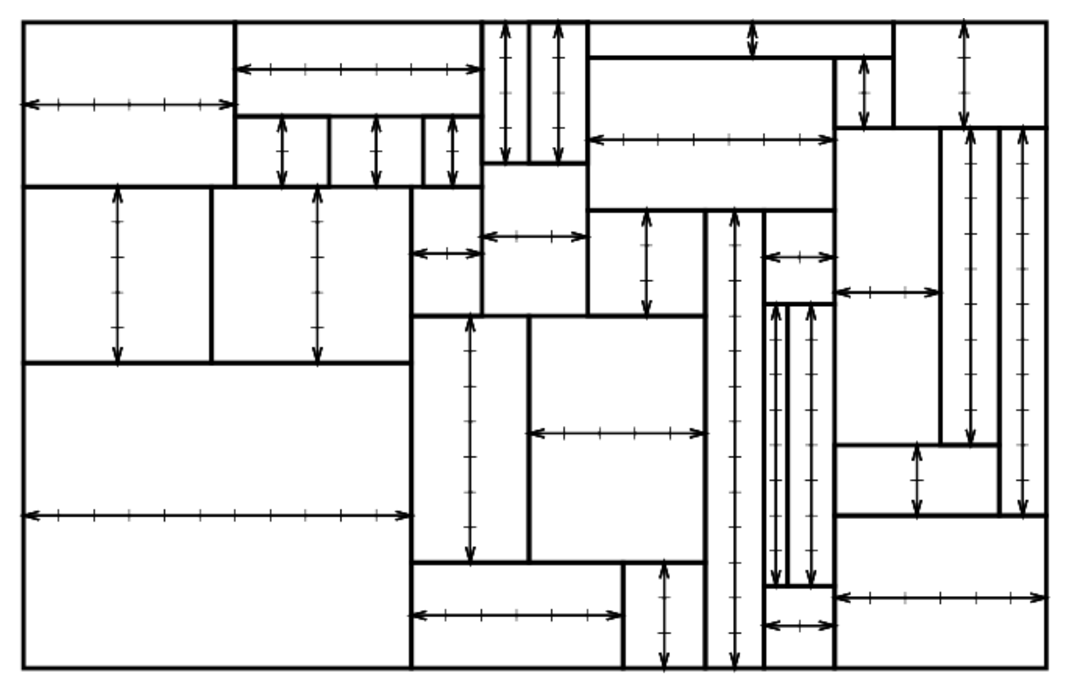
\includegraphics[scale=0.6]{Figs/Insight/rect}
\end{figure}

\subsection*{Весы и гири} %(TIPPING THE SCALES)

На столе у учителя стоят чашечные весы, правая чашка весов перевешивает.
На весах стоят гири не обязательно одного веса, на каждой из которых написаны фамилии одного \emph{или нескольких} учеников.
Ученик, входя в класс, переставляет на другую чашку весов каждую гирю, на которой написана его фамилия.
Докажите, что можно впустить в класс таких учеников, чтобы в результате перевесила левая чашка весов.

\subsection*{Часы на столе} %(WATCHERS ON THE TABLE)

На столе лежат пятьдесят точных ручных часов.
Докажите, что существует момент времени, когда сумма расстояний от центра стола до кончиков минутных стрелок больше, чем сумма расстояний от центра стола до центров часов.

\subsection*{Путь по шахматной доске} %(PATH ON CHESSBOARD)

Алиса начинает игру и ставит фишку в угол шахматной доски размером $n{\times}n$ клеток.
Боб передвигает фишку на соседнее поле, имеющее общую сторону с тем, на котором стоит фишка.
Второй раз ходить на поле, где уже побывала фишка, нельзя. 
Алиса и Боб ходят по очереди.
Проигрывает тот, кому некуда ходить.

При каких $n$ у Алисы есть выигрышная стратегия? 
При каких $n$ она выигрывает, если её первый ход не на угловое поле, а на соседнее с ним?

\subsection*{Степень в степени} %(EXPONENT UPON EXPONENT)

На экзамене по математике для старших классов Американской школы 1960-х годов 
был следующий вопрос:
Если 
$$x^{x^{x^{{\cdot}^{\cdot^{\cdot}}}}}=2$$
Чему равен $x$? 
Предполагаемое решение основывается на том, что степень «нижнего» $x$ равна всему выражению, таким образом $x^2\z=2$ и $x=\sqrt{2}$.
Но один ученик заметил, что если бы в задаче спрашивалось решение
$$x^{x^{x^{{\cdot}^{\cdot^{\cdot}}}}}=4$$
то он бы получил тот же ответ: $x=\sqrt[4]{4}=\sqrt{2}$

Хмм...
Чему же тогда равно ${\sqrt{2}}^{{\sqrt{2}}^{{\sqrt{2}}^{{\cdot}^{\cdot^{\cdot}}}}}$? 
Можете это доказать?

\subsection*{Солдаты в поле} %(SOLDIERS IN THE FIELD)

Нечётное число солдат расположилось на поле таким образом, что все попарные расстояния между ними (между каждой парой солдат) различны.
При этом каждый солдат должен присматривать за ближайшим к нему другим солдатом.

Докажите, что существует хотя бы один солдат, за которым никто не присматривает.

\subsection*{Отрезки и расстояния} %(INTERVALS AND DISTANCES)

Пусть множество $S$ состоит из $k$ непересекающихся отрезков, лежащих в единичном отрезке $[0,1]$.
Предположим, что $S$ обладает следующим свойством: для любого вещественного числа $d$ из отрезка $[0,1]$, в множестве $S$ существуют две точки на расстоянии $d$ друг от друга.
Докажите, что сумма длин отрезков $S$ не меньше $1/k$.

 
\subsection*{Собрать 15} %(SUMMING TO 15)

Алиса и Боб по очереди выбирают число из $1, 2,\dots,9$, без повторов.
Выигрывает тот, кто первый наберёт три числа, дающие в сумме 15.
Имеется ли у Алисы (она ходит первая)
выигрышная стратегия?
